\documentclass[preprint,12pt]{elsarticle}

\usepackage{amssymb}
\usepackage{amsmath}
\usepackage{booktabs}
\usepackage{url}
\usepackage{graphicx}

\journal{Engineering Applications of Artificial Intelligence}

\begin{document}

\begin{frontmatter}

\title{Risk-Aware Selective Inference for Resource-Constrained Industrial Anomaly Detection}

\author[guangxi]{Jin Huang\corref{cor1}}
\ead{614938561@qq.com}
\ead[url]{https://orcid.org/0009-0005-7489-2018}

\author[shangqiu]{Yubo Zhou}
\ead{surpass5837@163.com}

\cortext[cor1]{Corresponding author.}

\affiliation[guangxi]{organization={Guangxi Vocational Normal University},
            city={Nanning},
            postcode={530000},
            state={Guangxi},
            country={China}}

\affiliation[shangqiu]{organization={Shangqiu University},
            addressline={66 Beihai East Road, Liangyuan District},
            city={Shangqiu},
            postcode={476000},
            state={Henan},
            country={China}}

\begin{abstract}
Industrial anomaly detection systems must process many normal samples while allocating detailed analysis to the relatively small number of samples that may contain subtle defects. Applying a high-cost local detector to every image provides a strong accuracy reference but wastes computation on easy cases; random escalation controls the computation budget but does not use sample-specific risk. Here we study whether a low-cost global risk score can allocate a high-cost local patch-memory detector more effectively than random escalation under an exactly matched fallback budget. The proposed two-stage system first extracts a low-resolution global representation with an ImageNet-pretrained ResNet-18 and then escalates only high-risk samples to a higher-resolution local patch-memory path. The routing threshold is calibrated using normal images only. On the 15 categories of MVTec AD with three random seeds, risk-aware routing achieved a mean image-level AUROC of 0.8674 and Recall@5\%FPR of 0.7251, compared with 0.7796 and 0.6204 for a random controller with exactly the same number of escalated samples. The paired bootstrap differences were +0.0879 (95\% CI, 0.0676--0.1081) for AUROC and +0.1047 (95\% CI, 0.0754--0.1337) for Recall@5\%FPR. The advantage remained at target budgets of 10\%, 25\% and 40\%. A unified batch-one CUDA benchmark showed that the selective pipeline does not reduce per-sample P95 latency relative to the full detector; its benefit is instead the preferential allocation of expensive analysis to high-risk samples. These results establish a bounded systems contribution: risk-aware escalation improves the quality of budgeted industrial anomaly detection over matched random escalation, while its applicability is limited by distribution shift, routing errors and sequential two-stage execution.
\end{abstract}

\begin{highlights}
\item A two-stage industrial anomaly detector combines fast global screening with local patch-memory analysis.
\item Risk-aware escalation is compared with random escalation using exactly matched fallback counts.
\item Risk routing improves AUROC by 0.0879 over matched random routing on MVTec AD.
\item The advantage persists at 10\%, 25\% and 40\% calibration budgets.
\item The measured benefit is budget allocation, not lower sequential single-sample P95 latency.
\end{highlights}

\begin{keyword}
industrial anomaly detection \sep selective inference \sep risk-aware routing \sep patch-memory detection \sep resource-constrained inference \sep MVTec AD
\end{keyword}

\end{frontmatter}

\section{Introduction}

Industrial visual inspection combines a large stream of normal products with a small and heterogeneous set of defective products. Most normal images are visually simple, whereas subtle texture defects, small local changes and boundary anomalies may require higher-resolution feature extraction and local comparison. A detector that applies detailed analysis to every image can provide high accuracy, but its computational cost is incurred even when the image is easy. Conversely, a uniformly lightweight detector reduces computation but may miss anomalies that are not well represented by global features.

This creates a selective inference problem. The central question is not only which detector is more accurate, but also which samples should receive additional computation. A practical system should use a low-cost path to estimate sample risk and reserve a high-cost path for samples that are likely to benefit from further analysis. The difficulty is that a reported improvement can be confounded by the number of samples sent to the high-cost detector. A fair evaluation therefore requires a control that escalates exactly the same number of samples but selects them independently of the risk score.

In this work, we develop and evaluate a risk-aware two-stage anomaly detection system. The fast path uses low-resolution global features to produce a normality-based risk score. Samples above a threshold calibrated on normal images are escalated to a high-resolution local patch-memory detector. We compare this system with a random controller whose fallback count is matched exactly to the risk-aware system for every category and seed. This comparison isolates the value of selecting which samples receive expensive analysis.

Across 45 category--seed units on MVTec AD, the risk-aware controller improved AUROC in 35 units and Recall@5\%FPR in 36 units. The pooled mean AUROC was 0.8674 for risk-aware routing and 0.7796 for matched random routing. The corresponding recall values were 0.7251 and 0.6204. The advantage was observed at three budget settings, indicating that it was not caused by a single threshold choice.

The contribution is deliberately bounded. The proposed system does not replace the full detector, and it does not claim to reduce end-to-end single-sample P95 latency. In the measured sequential implementation, the risk-aware pipeline had a P95 latency of 16.47~ms, compared with 10.52~ms for the full path. The contribution is therefore a budget--quality allocation mechanism: under a fixed number of expensive fallbacks, risk-based selection produces better detection performance than random selection.

The contributions are:
\begin{enumerate}
\item a two-stage industrial anomaly detection pipeline that combines a low-cost global risk scorer with a high-cost local patch-memory detector;
\item an exactly matched random-escalation protocol that separates the value of risk-based selection from the value of using additional computation;
\item a multi-seed and multi-budget evaluation covering image-level detection, localising capability of the full path, and unified CUDA latency; and
\item an explicit analysis of routing errors, normal-distribution shift and the latency cost of sequential execution.
\end{enumerate}

\section{Related work}

Industrial anomaly detection is commonly formulated as learning the distribution of normal samples and identifying deviations at test time. Feature-memory methods compare test representations with stored normal representations and can use normal-only training data while retaining local spatial information \cite{mvtec,patchcore}. Gaussian feature-distribution methods such as PaDiM model local feature statistics and provide a complementary reference based on parametric normality modelling \cite{padim}. These methods typically define one inference path for every image. Our work does not propose a new patch-memory detector; instead, it studies how a fast global path can decide which inputs should receive an existing high-cost local analysis.

Selective prediction allocates model computation or abstention decisions according to input difficulty, uncertainty or estimated error risk \cite{selective}. Conditional computation has also been used to activate different network components or resolutions for different inputs \cite{conditional}. Industrial anomaly detection adds two constraints: training often uses only normal images, and the evaluation must distinguish risk-based selection from simply increasing the fraction of samples processed by an expensive model. We address these constraints with normal-only threshold calibration and an exact-count random control.

\section{Method}

\subsection{Problem formulation}

Let $x$ denote an input image. The system contains a fast detector $f_s$, a local detector $f_f$, and a binary routing function $r$. The fast detector produces a global anomaly score $s_s(x)$. The route decision is
\begin{equation}
r(x)=\mathbb{1}[s_s(x)\geq\tau],
\end{equation}
where $\tau$ is estimated from normal calibration images. The final score is
\begin{equation}
s(x)=(1-r(x))s_s(x)+r(x)s_f(x),
\end{equation}
where $s_f(x)$ is the local patch-memory score. The route is a selective replacement of the fast score, not an ensemble average of the two scores.

For every category and seed, the matched random controller uses the same number of escalated test images as the risk-aware controller. It samples the escalated images without replacement using a fixed seed and leaves detector outputs unchanged. The primary comparison therefore holds the fallback count constant and changes only the selection rule.

\subsection{Fast global path}

The fast path resizes each image to $128\times128$ pixels and extracts the layer-2 feature map of an ImageNet-pretrained ResNet-18. Spatial average pooling followed by $L_2$ normalisation produces a global descriptor $z_s(x)$. Descriptors from normal training images form a normal memory bank $\mathcal{M}_s$. The fast anomaly score is
\begin{equation}
s_s(x)=\min_{z\in\mathcal{M}_s}\|z_s(x)-z\|_2.
\end{equation}

\subsection{High-cost local patch-memory path}

The local path resizes each image to $224\times224$ pixels and extracts layer-3 ResNet-18 patch descriptors. Each patch descriptor is normalised, and descriptors from all normal training images form a local memory bank $\mathcal{M}_f$. For each test patch, the detector computes the nearest-neighbour distance to $\mathcal{M}_f$. The image-level score is the mean of the largest 10\% of patch distances:
\begin{equation}
s_f(x)=\operatorname{MeanTop}_{10\%}\left(\left\{\min_{z\in\mathcal{M}_f}\|p_i(x)-z\|_2\right\}_i\right).
\end{equation}

The same patch-distance map can be upsampled to the input resolution for pixel-level localisation. In this study, the local path is a high-cost reference detector and the contribution is the routing mechanism around it.

\subsection{Normal-only calibration and budget control}

Normal training images are divided into a memory-bank subset and an independent calibration subset. No test labels are used to choose $\tau$. For a target calibration budget $b$, the threshold is the $(1-b)$-quantile of fast scores on the normal calibration subset. Because the normal distribution may shift between calibration and test traffic, the realised fallback rate is reported explicitly rather than treated as a guaranteed budget.

\section{Experimental setup}

\subsection{Dataset and protocol}

We use MVTec AD, which contains 15 object and texture categories with normal-only training images and defective test images \cite{mvtec}. Training uses only \texttt{train/good} images. The official test images are used for final evaluation. Results are macro-averaged over categories. The main study contains 15 categories $\times$ 3 seeds = 45 category--seed units.

The primary metrics are image-level AUROC and Recall@5\%FPR. For paired uncertainty estimates, category--seed units are resampled with replacement to obtain 95\% bootstrap confidence intervals for Risk minus Random.

\subsection{Compared systems}

We compare Fast only, Random matched fallback, Risk fallback and Full only. We additionally report a PaDiM-style diagonal-Gaussian baseline using the same layer-3 patch features. This implementation is a controlled reference and is not claimed to reproduce every component of the official PaDiM system.

\subsection{Statistical analysis}

Statistical analyses were performed with Python 3.12 and PyTorch 2.8.0 for model evaluation. The primary analysis unit was a category--seed unit: each of the 15 MVTec AD categories was evaluated with each of three seeds (17, 29 and 41), yielding 45 units. Image-level AUROC and Recall@5\%FPR were summarised as the mean across these units. The primary comparison was Risk versus Random with exactly matched fallback counts within each category--seed unit. Uncertainty was estimated by paired bootstrap resampling of the 45 category--seed units, and 95\% confidence intervals were calculated for the Risk-minus-Random difference. The 10\%, 25\% and 40\% budget sweep, pixel-level localisation audit and latency benchmark were treated as secondary descriptive analyses; no $p$-values or star-based significance labels are reported for these analyses. Latency was summarised by P50 and P95 over repeated batch-one CUDA measurements after warm-up and explicit CUDA synchronisation; repeated timing measurements were not treated as independent experimental units. No test labels were used for threshold calibration, and no observations were excluded from the formal evaluations.

\section{Results}

\subsection{Risk-aware selection improves detection under matched fallback counts}

Risk-aware routing improved performance over the matched random controller while using exactly the same number of escalated samples. The mean image-level AUROC was 0.8674 for Risk and 0.7796 for Random. Recall@5\%FPR was 0.7251 and 0.6204, respectively. The difference was +0.0879 AUROC points (95\% bootstrap CI, 0.0676--0.1081) and +0.1047 recall points (95\% bootstrap CI, 0.0754--0.1337). Risk improved AUROC in 35 of 45 category--seed units and recall in 36 of 45 units. Fallback counts matched exactly in all 45 units.

\begin{figure}[t]
\centering
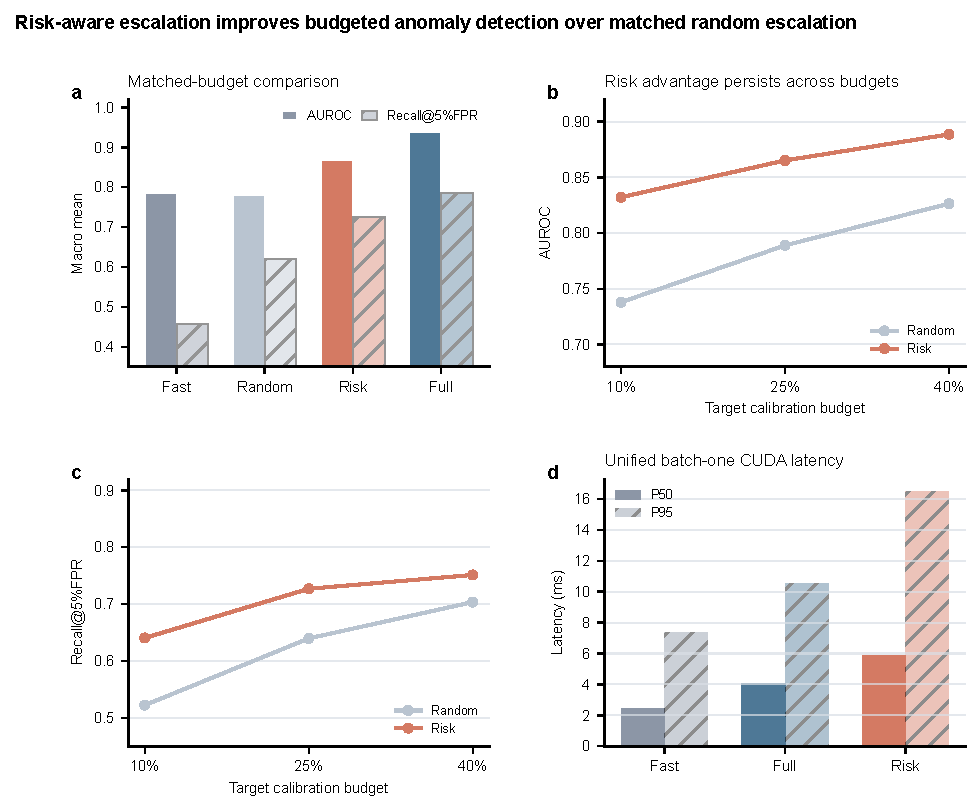
\includegraphics[width=0.98\textwidth]{figures/Fig1_main_results.pdf}
\caption{\textbf{Risk-aware escalation improves budgeted anomaly detection over matched random escalation.} (a) Macro-mean image-level AUROC and Recall@5\%FPR for Fast, Random matched fallback, Risk fallback and Full on MVTec AD. Values are means over 45 category--seed units (15 categories and three seeds). Random and Risk use the same realised fallback count. (b) AUROC across target calibration budgets for Random and Risk on seed 17 and 15 categories. (c) Recall@5\%FPR across the same budgets. (d) P50 and P95 end-to-end latency from the unified batch-one CUDA benchmark. Latency values are descriptive summaries of repeated measurements and are not treated as independent replicates. Summary source data are provided in \texttt{source\_data\_eaai\_figures.csv}, and unit-level source data are provided in \texttt{mvtec\_category\_seed\_unit\_results.csv}.}
\label{fig:main}
\end{figure}

\begin{table}[t]
\centering
\caption{Main image-level detection results on MVTec AD.}
\label{tab:main}
\begin{tabular}{lccc}
\toprule
Method & AUROC & Recall@5\%FPR & Fallback rate \\
\midrule
Fast only & 0.7860 & 0.4575 & 0.0000 \\
Random matched & 0.7796 & 0.6204 & 0.7197 \\
Risk fallback & \textbf{0.8674} & \textbf{0.7251} & 0.7197 \\
Full only & 0.9390 & 0.7852 & 1.0000 \\
\bottomrule
\end{tabular}
\end{table}

Full remained the strongest accuracy reference. Risk did not surpass Full; its demonstrated advantage is better selection than random escalation at the same realised fallback count. The PaDiM-style diagonal-Gaussian reference achieved mean AUROC 0.8982 and Recall@5\%FPR 0.6544 over the same 45 units.

\begin{figure}[t]
\centering
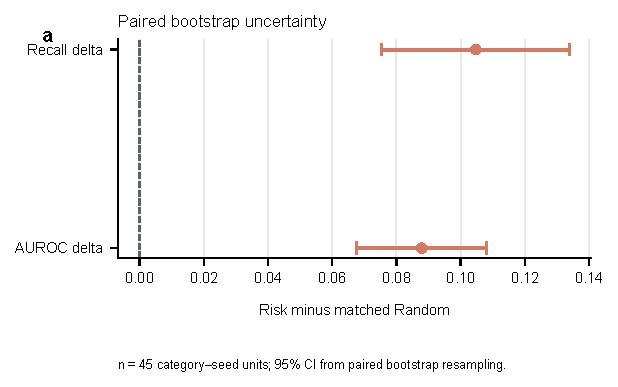
\includegraphics[width=0.72\textwidth]{figures/Fig2_risk_random_uncertainty.pdf}
\caption{\textbf{Paired bootstrap uncertainty for risk-aware routing.} Risk-minus-Random differences in AUROC and Recall@5\%FPR. Points show the observed mean difference over 45 category--seed units; horizontal bars show 95\% confidence intervals from paired bootstrap resampling of those units. The vertical dashed line marks zero. Summary source data and the per-unit values used to recompute the intervals are provided in the accompanying source-data files.}
\label{fig:uncertainty}
\end{figure}

\subsection{Budget sensitivity}

Risk-aware selection remained better than matched random selection at all three evaluated target budgets. At 10\%, Risk achieved AUROC 0.8322 and Recall@5\%FPR 0.6404, compared with 0.7379 and 0.5222 for Random. At 25\%, the corresponding values were 0.8652 and 0.7269 versus 0.7889 and 0.6396. At 40\%, Risk achieved 0.8886 and 0.7512 versus 0.8264 and 0.7035.

\begin{table}[t]
\centering
\caption{Budget sensitivity on seed 17 across the 15 MVTec AD categories.}
\label{tab:budget}
\begin{tabular}{lccccc}
\toprule
Target & Random AUROC & Risk AUROC & Random Recall & Risk Recall & Risk fallback \\
\midrule
10\% & 0.7379 & \textbf{0.8322} & 0.5222 & \textbf{0.6404} & 0.5757 \\
25\% & 0.7889 & \textbf{0.8652} & 0.6396 & \textbf{0.7269} & 0.7223 \\
40\% & 0.8264 & \textbf{0.8886} & 0.7035 & \textbf{0.7512} & 0.8217 \\
\bottomrule
\end{tabular}
\end{table}

\subsection{Localisation and latency boundary}

The full local path achieved mean pixel-level AUROC 0.9543 and mean PRO 0.8380 at FPR 0.30 over the 15 categories. These measurements establish the spatial detection capability of the local path; they do not establish that every sample routed by Risk receives a localisation map.

In the unified batch-one CUDA benchmark, Fast, Full and Risk achieved P50/P95 latencies of 2.44/7.35~ms, 4.09/10.52~ms and 5.85/16.47~ms, respectively. Risk was slower in end-to-end P95 because it first computes the fast path and then executes the local path for selected samples. The current implementation therefore does not support a claim of lower per-sample P95 latency.

\section{Discussion}

The results show that the selection rule can matter as much as the fallback count in a two-stage anomaly detector. When the number of expensive local evaluations is held fixed, selecting samples by a fast normality-based risk score is more effective than selecting them randomly. The result is supported by exact per-unit matching, three random seeds, paired bootstrap intervals and a three-point budget sweep.

The evidence also clarifies what the system does not solve. The Full detector remains more accurate because every image receives local analysis. The sequential Risk implementation is not faster in single-sample P95 because routing requires the fast computation before the local computation. A production deployment would therefore need throughput-oriented batching, asynchronous scheduling, a calibrated budget controller, or a genuinely cheaper local kernel before claiming an end-to-end latency advantage.

The current novelty is best understood as a system-level resource allocation mechanism around a normal-memory anomaly detector. It is not a new backbone, a new PatchCore formulation or a learned uncertainty model. The main applicability boundary is that the evidence comes from MVTec AD, risk ranking can miss purely local defects, and distribution shift can increase the realised fallback rate.

\section{Conclusion}

We presented a risk-aware selective inference system for industrial anomaly detection. On MVTec AD, Risk-aware routing outperformed an exactly matched random controller across image-level AUROC, Recall@5\%FPR and three budget settings. The evidence supports a specific conclusion: risk-based allocation of expensive anomaly analysis is more effective than random allocation under the same realised fallback count. The evidence does not support claims that the system surpasses the Full detector or reduces sequential single-sample P95 latency.

\section*{Data and code availability}

The study uses the publicly available MVTec AD dataset. The exact data split, calibration protocol, route seeds, result files and evaluation scripts should be deposited in a public repository before submission. \textbf{Author action: insert repository URL, software version and dataset access statement.}

\section*{Declaration of competing interests}

The authors declare no competing interests.

\begin{thebibliography}{00}

\bibitem{mvtec}
Paul Bergmann, Michael Fauser, David Sattlegger, Carsten Steger,
MVTec AD---A comprehensive real-world dataset for unsupervised anomaly detection,
in: Proceedings of the IEEE/CVF Conference on Computer Vision and Pattern Recognition, 2019.

\bibitem{patchcore}
Karsten Roth, Lars Hickmann, Sebastian Schuler, et al.,
Towards total recall in industrial anomaly detection,
in: Proceedings of the IEEE/CVF Conference on Computer Vision and Pattern Recognition, 2022.

\bibitem{padim}
Thomas Defard, Aleksandr Setkov, Angelique Loesch, Romaric Audigier,
PaDiM: A patch distribution modeling framework for anomaly detection and localization,
in: Pattern Recognition. ICPR International Workshops and Challenges, 2021.

\bibitem{selective}
Yonatan Geifman, Ran El-Yaniv,
Selective classification for deep neural networks,
in: Advances in Neural Information Processing Systems, 2017.

\bibitem{conditional}
David E. Bengio, Nicholas Léonard, Aaron Courville,
Estimating or propagating gradients through stochastic neurons for conditional computation,
arXiv:1308.3432, 2013.

\end{thebibliography}

\end{document}
